\section{Experiment=25: convection in a box, BA vs EBA}

This experiment is very similar to the convection experiment of \textcite{blbc89}.
Free slip boundary conditions are applied on all sides.
The main difference resides in the fact that all physical parameters are Earth-like
and borrowed from \textcite{lee_13}:

\begin{lstlisting}
Lx = 1000e3
Lz = 1000e3
g0 = 10 
Ttop = 0 + 273 
Tbottom = 3000 +273 
alphaT = 3.125e-5  # thermal expansion coefficient
rho0 = 4000 # reference density
hcapa = 1250  # heat capacity
kappa=1e-6
hcond=kappa*rho0*hcapa
eta0 = 3.750e23 # Ra=1e4
\end{lstlisting}
By choosing these parameters we can make sure that the Rayleigh number, the 
thermal diffusivity and the dissipation number are assigned the desired value:
\begin{lstlisting}
Di = alphaT * g0 * Lz / hcapa
kappa = hcond / rho0 / hcapa
Ra = alphaT * rho0 * g0 * (Lz**3) * (Tbottom - Ttop) / kappa / eta0
\end{lstlisting}
which yields
\begin{verbatim}
-> Di= 0.25
-> kappa= 1e-06
-> Ra= 10000.000000000002
\end{verbatim}

In all the following figures time is rendered dimensionless by diving 
it by the ref time. Reference velocity and pressure values are also 
taken from \textcite{kilv10}:
\begin{lstlisting}
reftime=rho0*hcapa*Lz**2/hcond 
refvel=Lz/reftime 
refPress = eta0 * hcond / rho0 / hcapa / Lz**2
refTemp = Tbottom - Ttop
\end{lstlisting}
which gives (for $Ra=10^4$):
\begin{verbatim}
-> reftime 1.000000e+18 s | 3.168809e+10 yr
-> refvel 1.000000e-12 m/s | 3.155760e-03 cm/yr
-> refPress 3.750000e+05 
\end{verbatim}
The material model is then very simple:
\begin{verbatim}
swarm_rho[:] = rho0 * (1 - alphaT * (swarm_T[:]-Ttop))
swarm_eta[:] = eta0
swarm_hcond[:] = hcond
swarm_hcapa[:] = hcapa
swarm_hprod[:] = 0
swarm_alpha[:] = alphaT
\end{verbatim}


I have also built this experiment with ASPECT and the results obtained with 
MEEUUW are compared with those of ASPECT in what follows.


The article by \textcite{lee_13} is precious because it 
shows the temperature field and implicitely the used boundary 
conditions at the top and bottom. These are important for hte 
EBA formulation cases.
Note that it unfortunately does not report on the rms velocity.

A remark about a lesson learned the hard way: As explained in 
the ASPECT manual\footnote{\url{https://aspect-documentation.readthedocs.io/en/latest/user/methods/basic-equations/adiabatic-heating.html}}
the adiabatic term is $\alpha T Dp/Dt$ where $Dp/Dt$ is the material derivative, i.e.
\[
\frac{Dp}{Dt} = \frac{\partial p}{\partial t} + \vec\upnu \cdot \vec\nabla p
\]
The time derivative is then neglected, and very often the pressure gradient is replaced by the 
gradient of the lithostatic pressure so that $ \vec\nabla p \sim - \rho \vec{g}$.
If we look closely at \textcite{kilv10} and \textcite{lee_13} we see that it is also their preference.
Spoiler alert, using the real pressure gradient actually leads to results that do not match 
those of these publications.

%-----------------------------------
\subsection{BA formulation - Ra=1e4}

%\begin{center}
%
\includegraphics[width=5.7cm]{exp25/BA/Nu.pdf}
%
\includegraphics[width=5.7cm]{exp25/BA/vrms.pdf}
%
\includegraphics[width=5.7cm]{exp25/BA/wag.pdf}
%
\includegraphics[width=5.7cm]{exp25/BA/tvd.pdf}
%
\includegraphics[width=5.7cm]{exp25/BA/kinetic_energy.pdf}
%
\includegraphics[width=5.7cm]{exp25/BA/Tavrg.pdf}
%\end{center}

\begin{center}
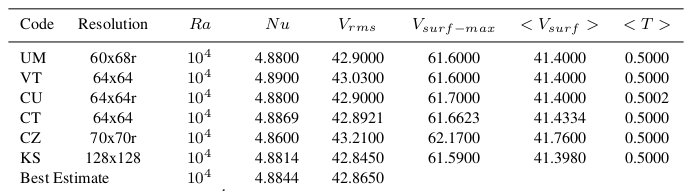
\includegraphics[width=11cm]{exp25/images/kilv10_BA}\\
Taken from \textcite{kilv10}.
\end{center}

\begin{center}
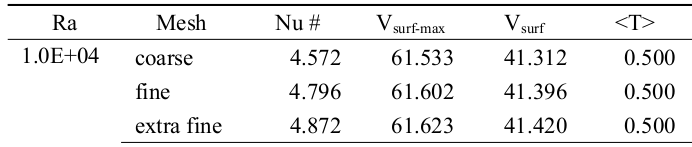
\includegraphics[width=8cm]{exp25/images/lee13_BA}\\
Taken from \textcite{lee_13}.
\end{center}

%-----------------------------------
\subsection{BA formulation - Ra=1e5}

\subsection{BA formulation - Ra=1e6}


\newpage
%---------------------------------------------
\subsection{EBA formulation - Ra=1e4, Di=0.25}

\begin{center}

\includegraphics[width=5.7cm]{exp25/Ra1e4/Nu.pdf}

\includegraphics[width=5.7cm]{exp25/Ra1e4/vrms.pdf}

\includegraphics[width=5.7cm]{exp25/Ra1e4/wag.pdf}

\includegraphics[width=5.7cm]{exp25/Ra1e4/tvd.pdf}
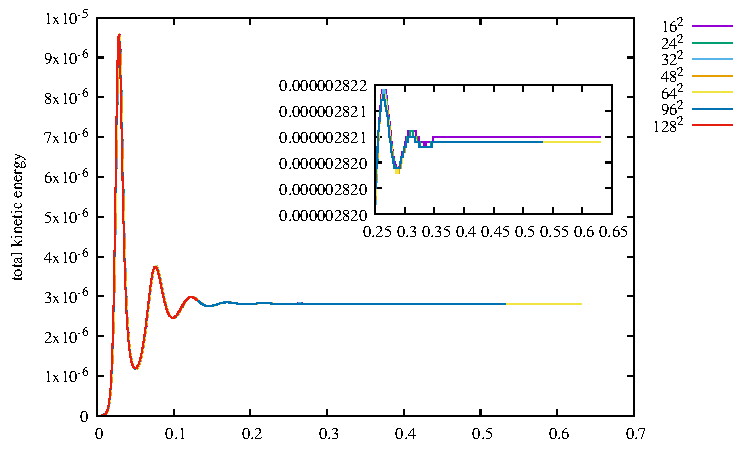
\includegraphics[width=5.7cm]{exp25/Ra1e4/kinetic_energy.pdf}

\includegraphics[width=5.7cm]{exp25/Ra1e4/Tavrg.pdf}
%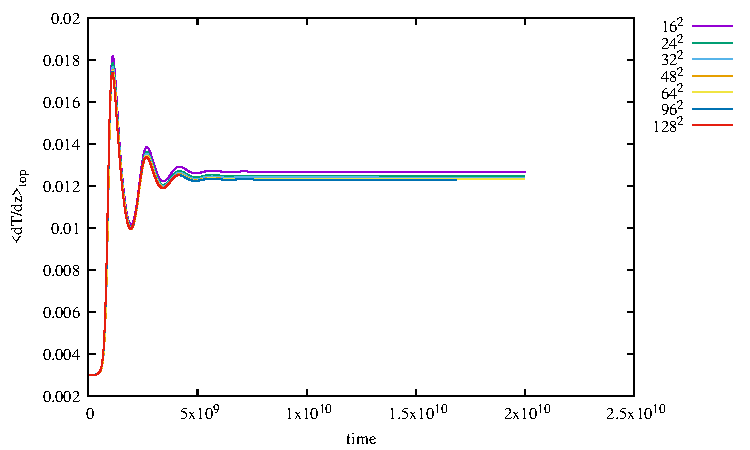
\includegraphics[width=5.7cm]{exp25/Ra1e4/avrg_dTdz_top.pdf}
%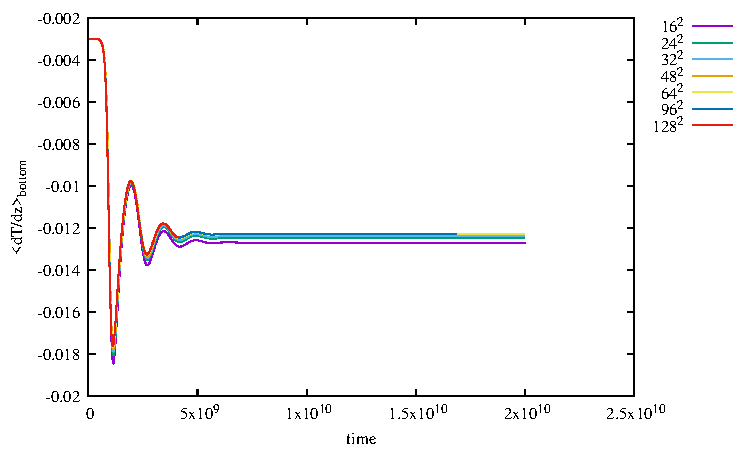
\includegraphics[width=5.7cm]{exp25/Ra1e4/avrg_dTdz_bottom.pdf}
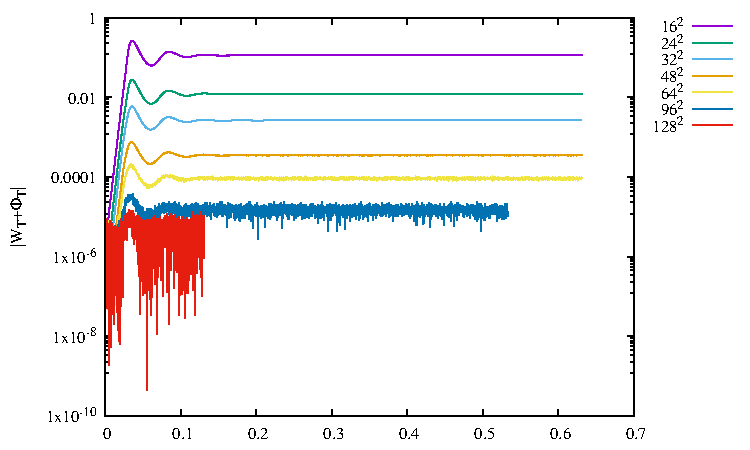
\includegraphics[width=5.7cm]{exp25/Ra1e4/delta.pdf}
\end{center}

\begin{center}
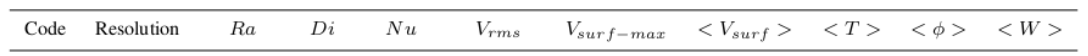
\includegraphics[width=13cm]{exp25/images/header}\\
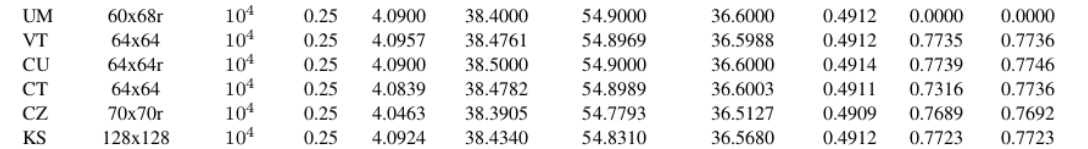
\includegraphics[width=13cm]{exp25/images/1e4}\\
Taken from \textcite{kilv10}.
\end{center}

\begin{center}
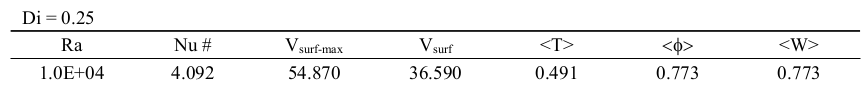
\includegraphics[width=13cm]{exp25/images/lee13_EBA}\\
Taken from \textcite{lee_13}.
\end{center}





\newpage
%---------------------------------------------
\subsection{EBA formulation - Ra=1e5, Di=0.25}

\begin{center}
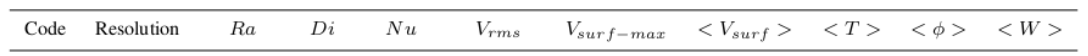
\includegraphics[width=13cm]{exp25/images/header}\\
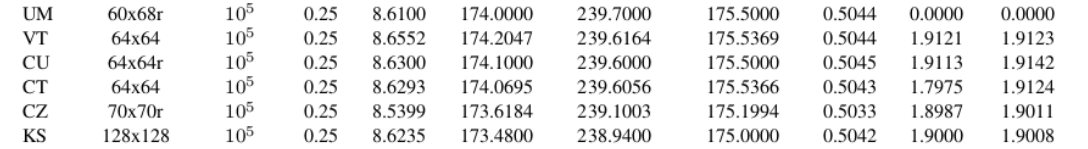
\includegraphics[width=13cm]{exp25/images/1e5}\\
Taken from \textcite{kilv10}.
\end{center}

\newpage
%---------------------------------------------
\subsection{EBA formulation - Ra=1e6, Di=0.25}

\begin{center}
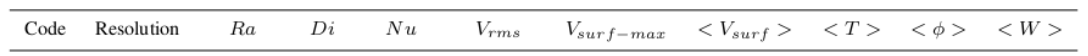
\includegraphics[width=13cm]{exp25/images/header}\\
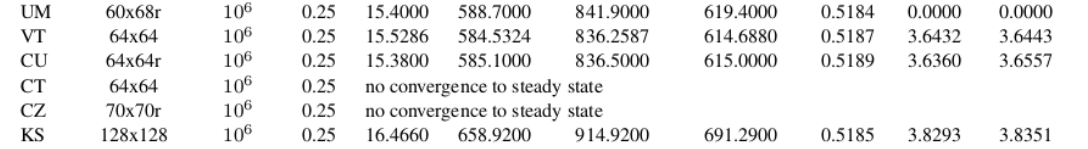
\includegraphics[width=13cm]{exp25/images/1e6}\\
Taken from \textcite{kilv10}.
\end{center}









%\begin{center}
%\includegraphics[width=13cm]{exp25/EBA/kilv10_eba}\\
%Taken from \textcite{kilv10} (2010).
%\end{center}
